\documentclass[10pt]{article}
\bibliographystyle{plain}
\usepackage[utf8]{inputenc}
\usepackage{graphicx}
\usepackage{caption}
\usepackage{subcaption}

%\usepackage{floatflt}
%\usepackage{wrapfig}
%\usepackage[innercaption]{sidecap}
%\usepackage{subfig}
%\usepackage{psfrag}
%\usepackage{amsmath}
\usepackage{geometry}
\geometry{inner=0.5cm, outer=0.5cm, bottom=2cm, top=1cm}

%\newcommand{\foldername}{fig}

%\def\foldername{../../Figures}
\def\foldername{../../Training_nStim1_nExcMpn800_nStates20_nActions21_it15-300/Figures}

%\date{\today}

\begin{document}

%\begin{figure}
%    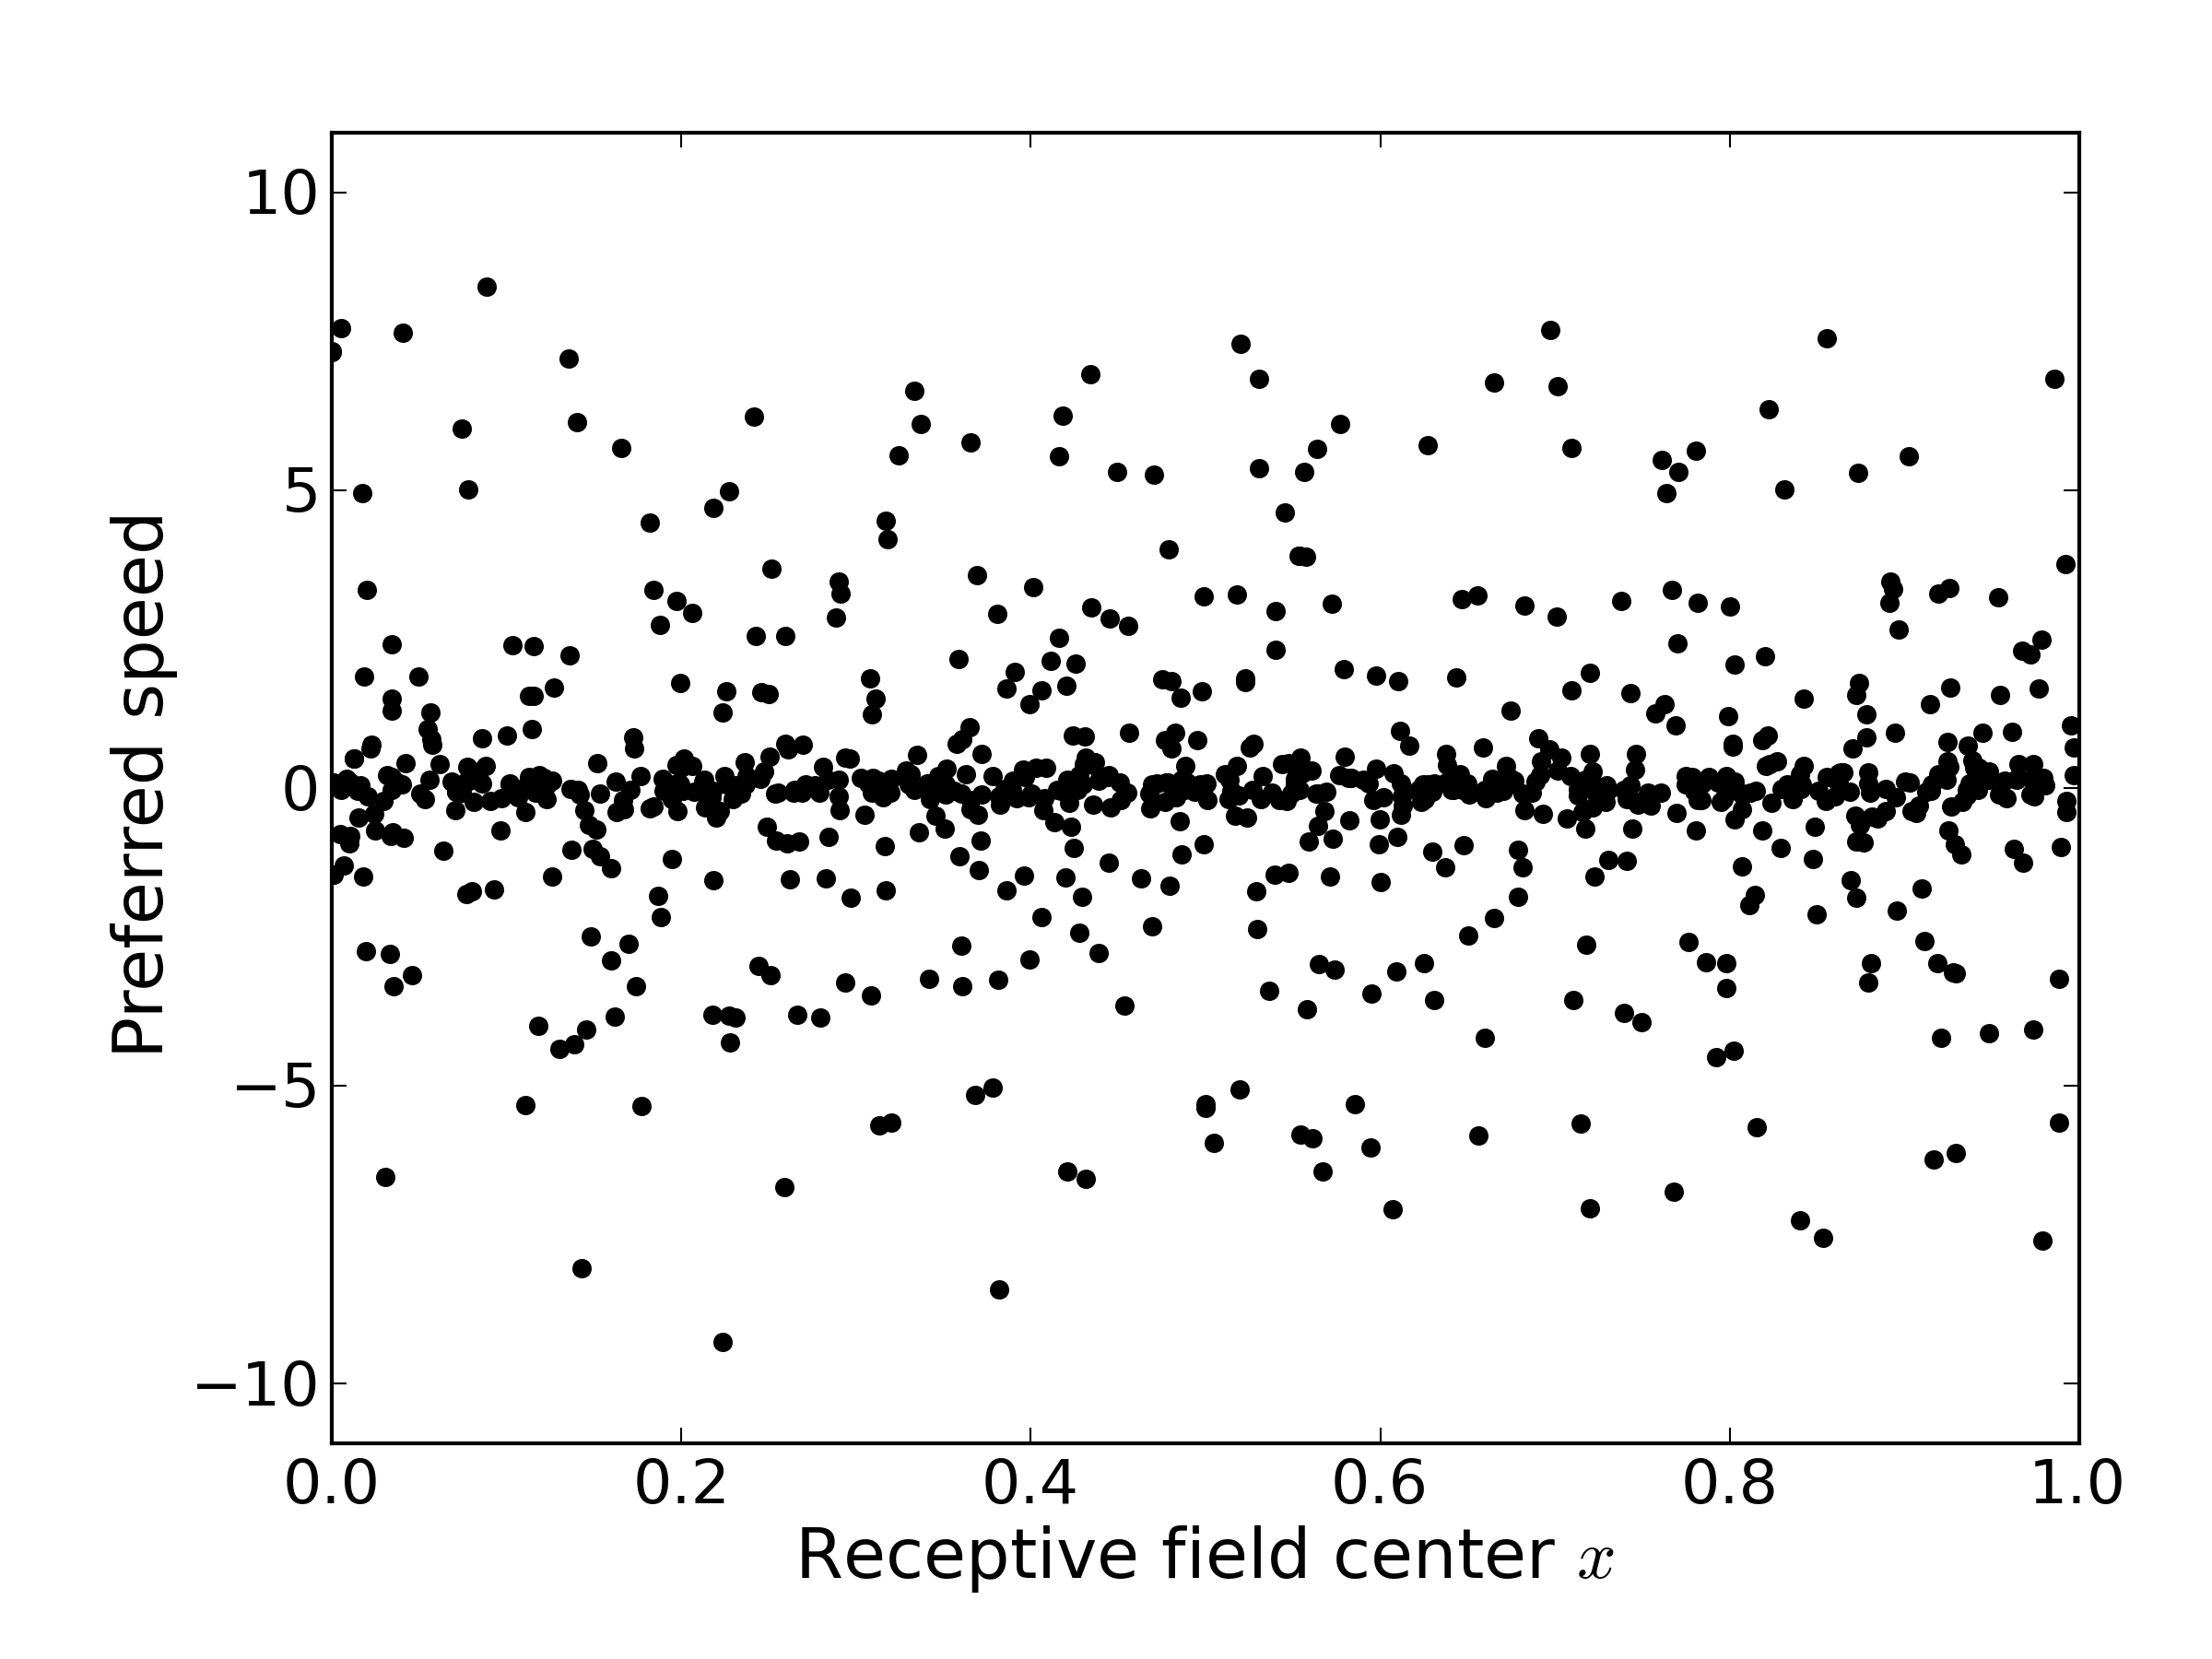
\includegraphics[width=0.8\textwidth]{\foldername/tuning_space}
%\end{figure}

%\begin{figure}
%    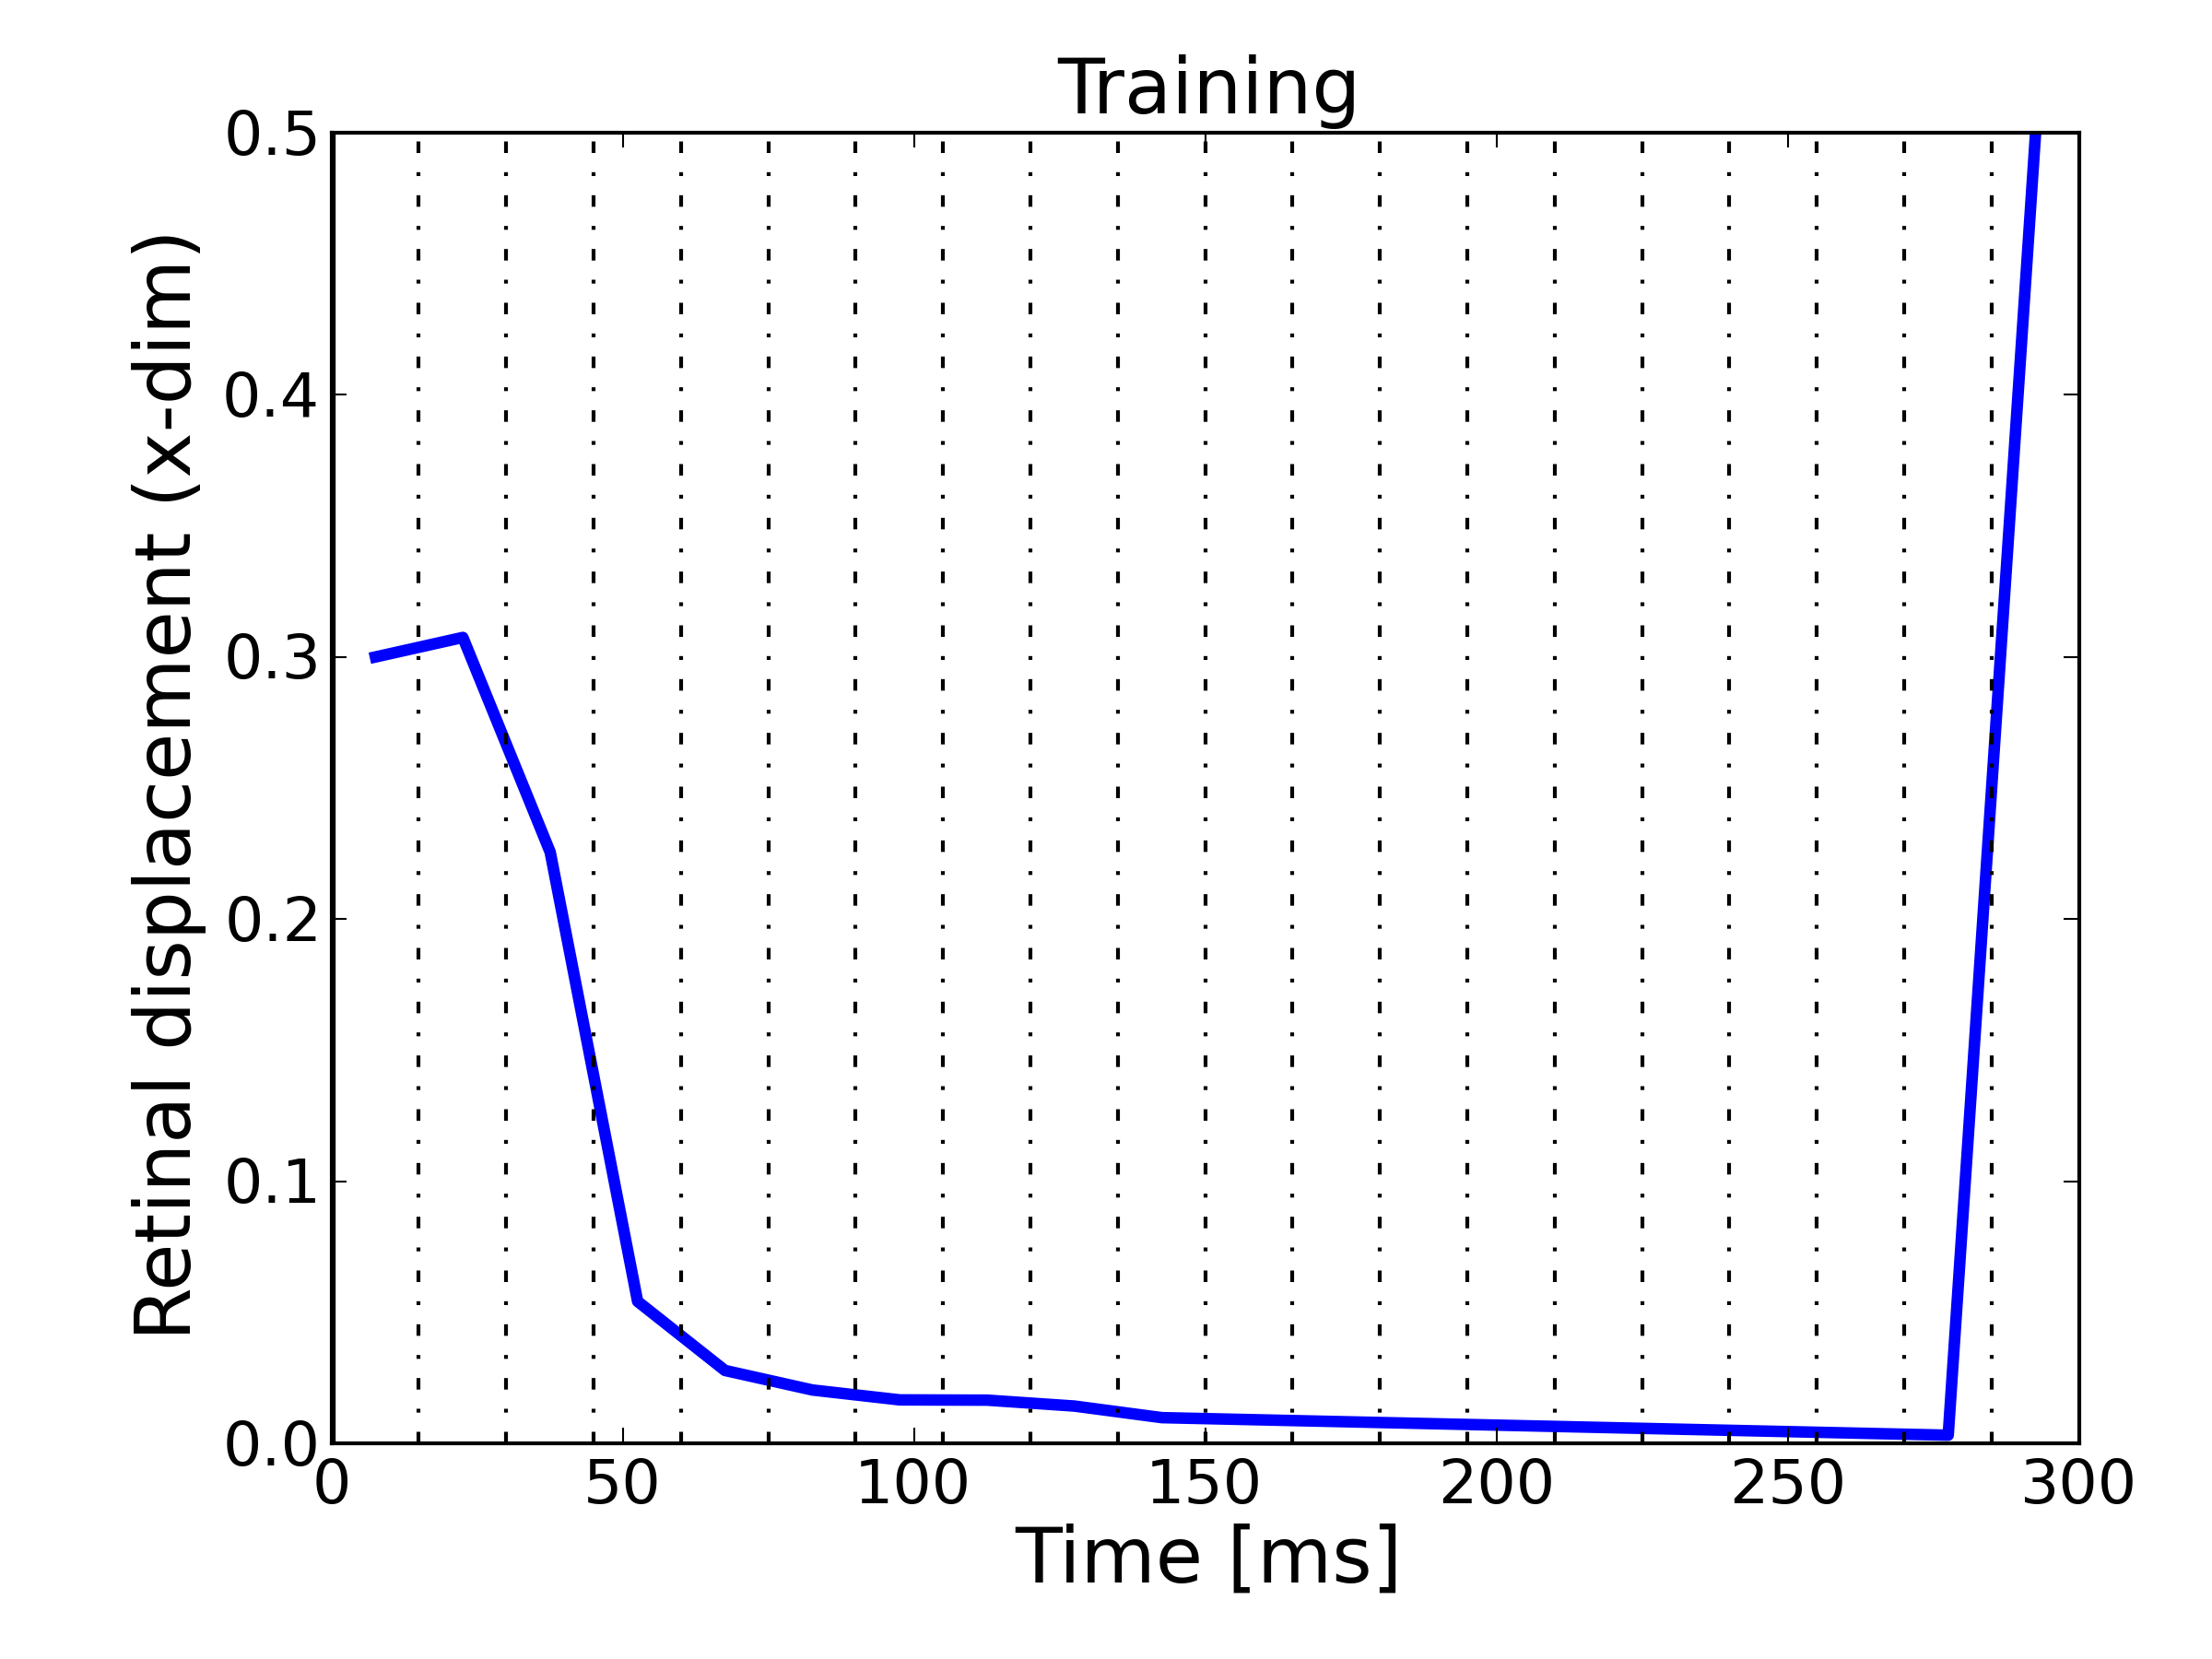
\includegraphics[width=0.8\textwidth]{\foldername/mpn_displacement}
%\end{figure}


%\begin{tabular}{cc}
%    \begin{figure} 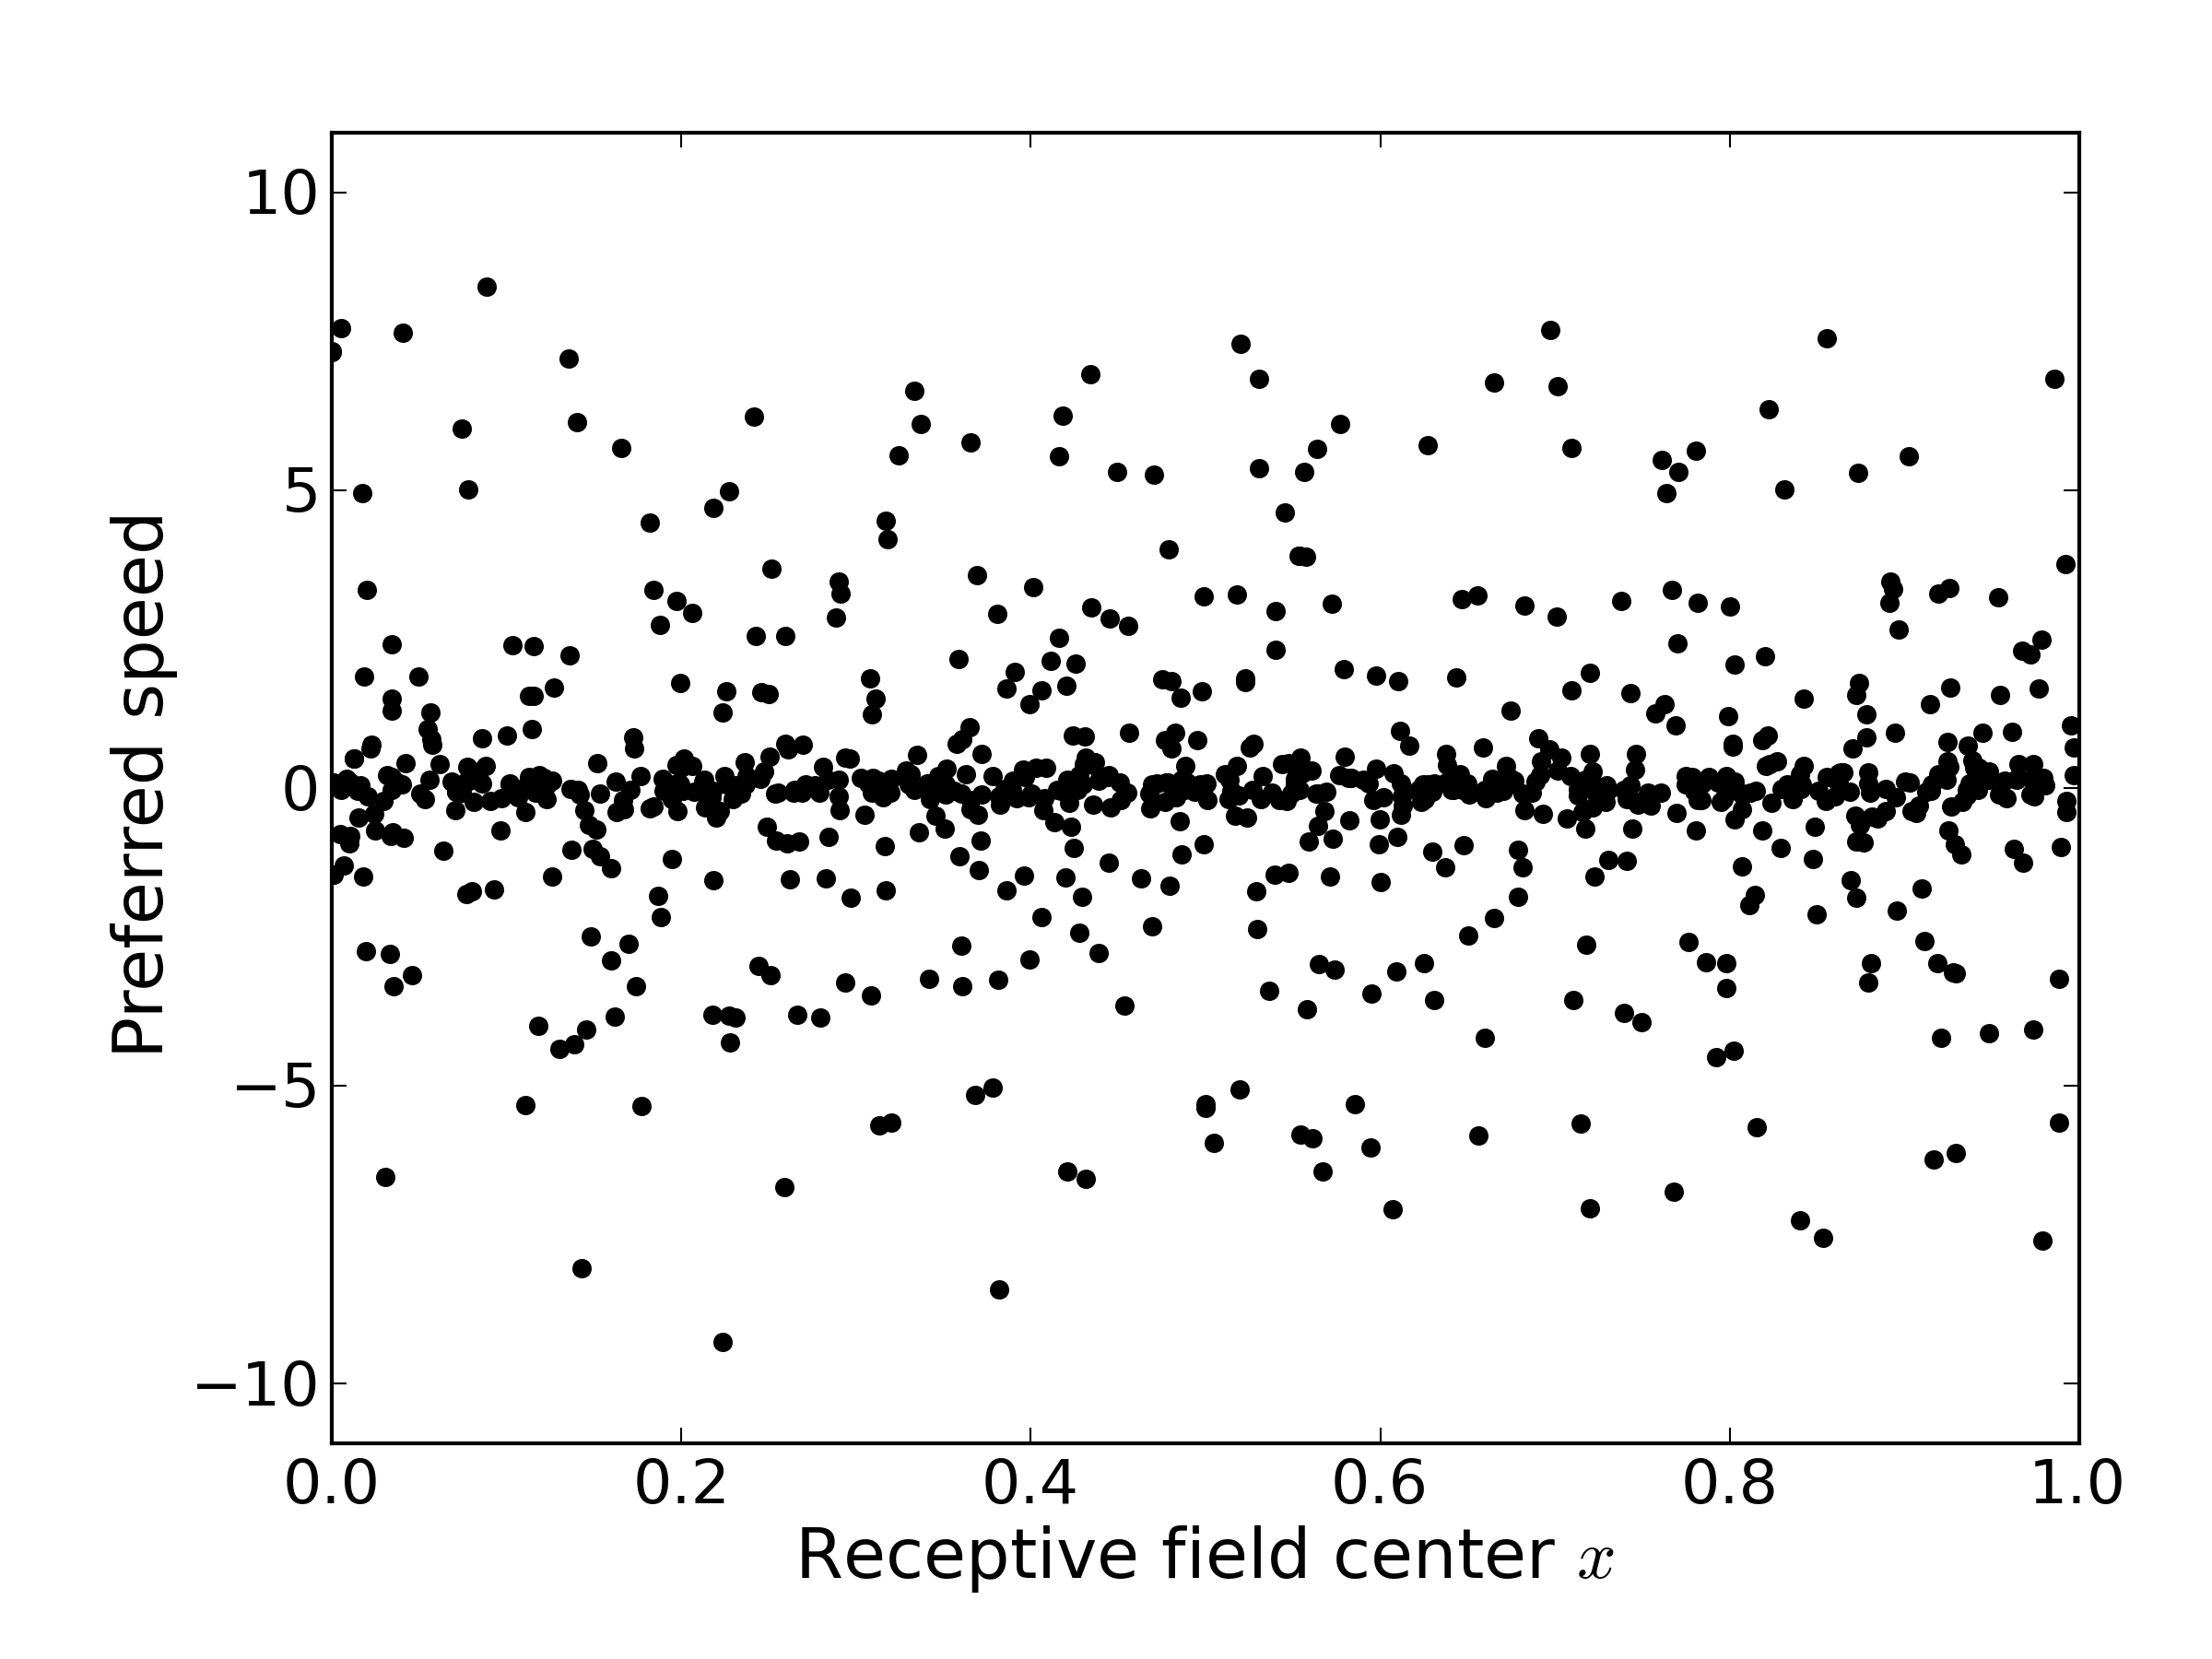
\includegraphics[width=0.4\textwidth]{\foldername/tuning_space} \end{figure} & \begin{figure} 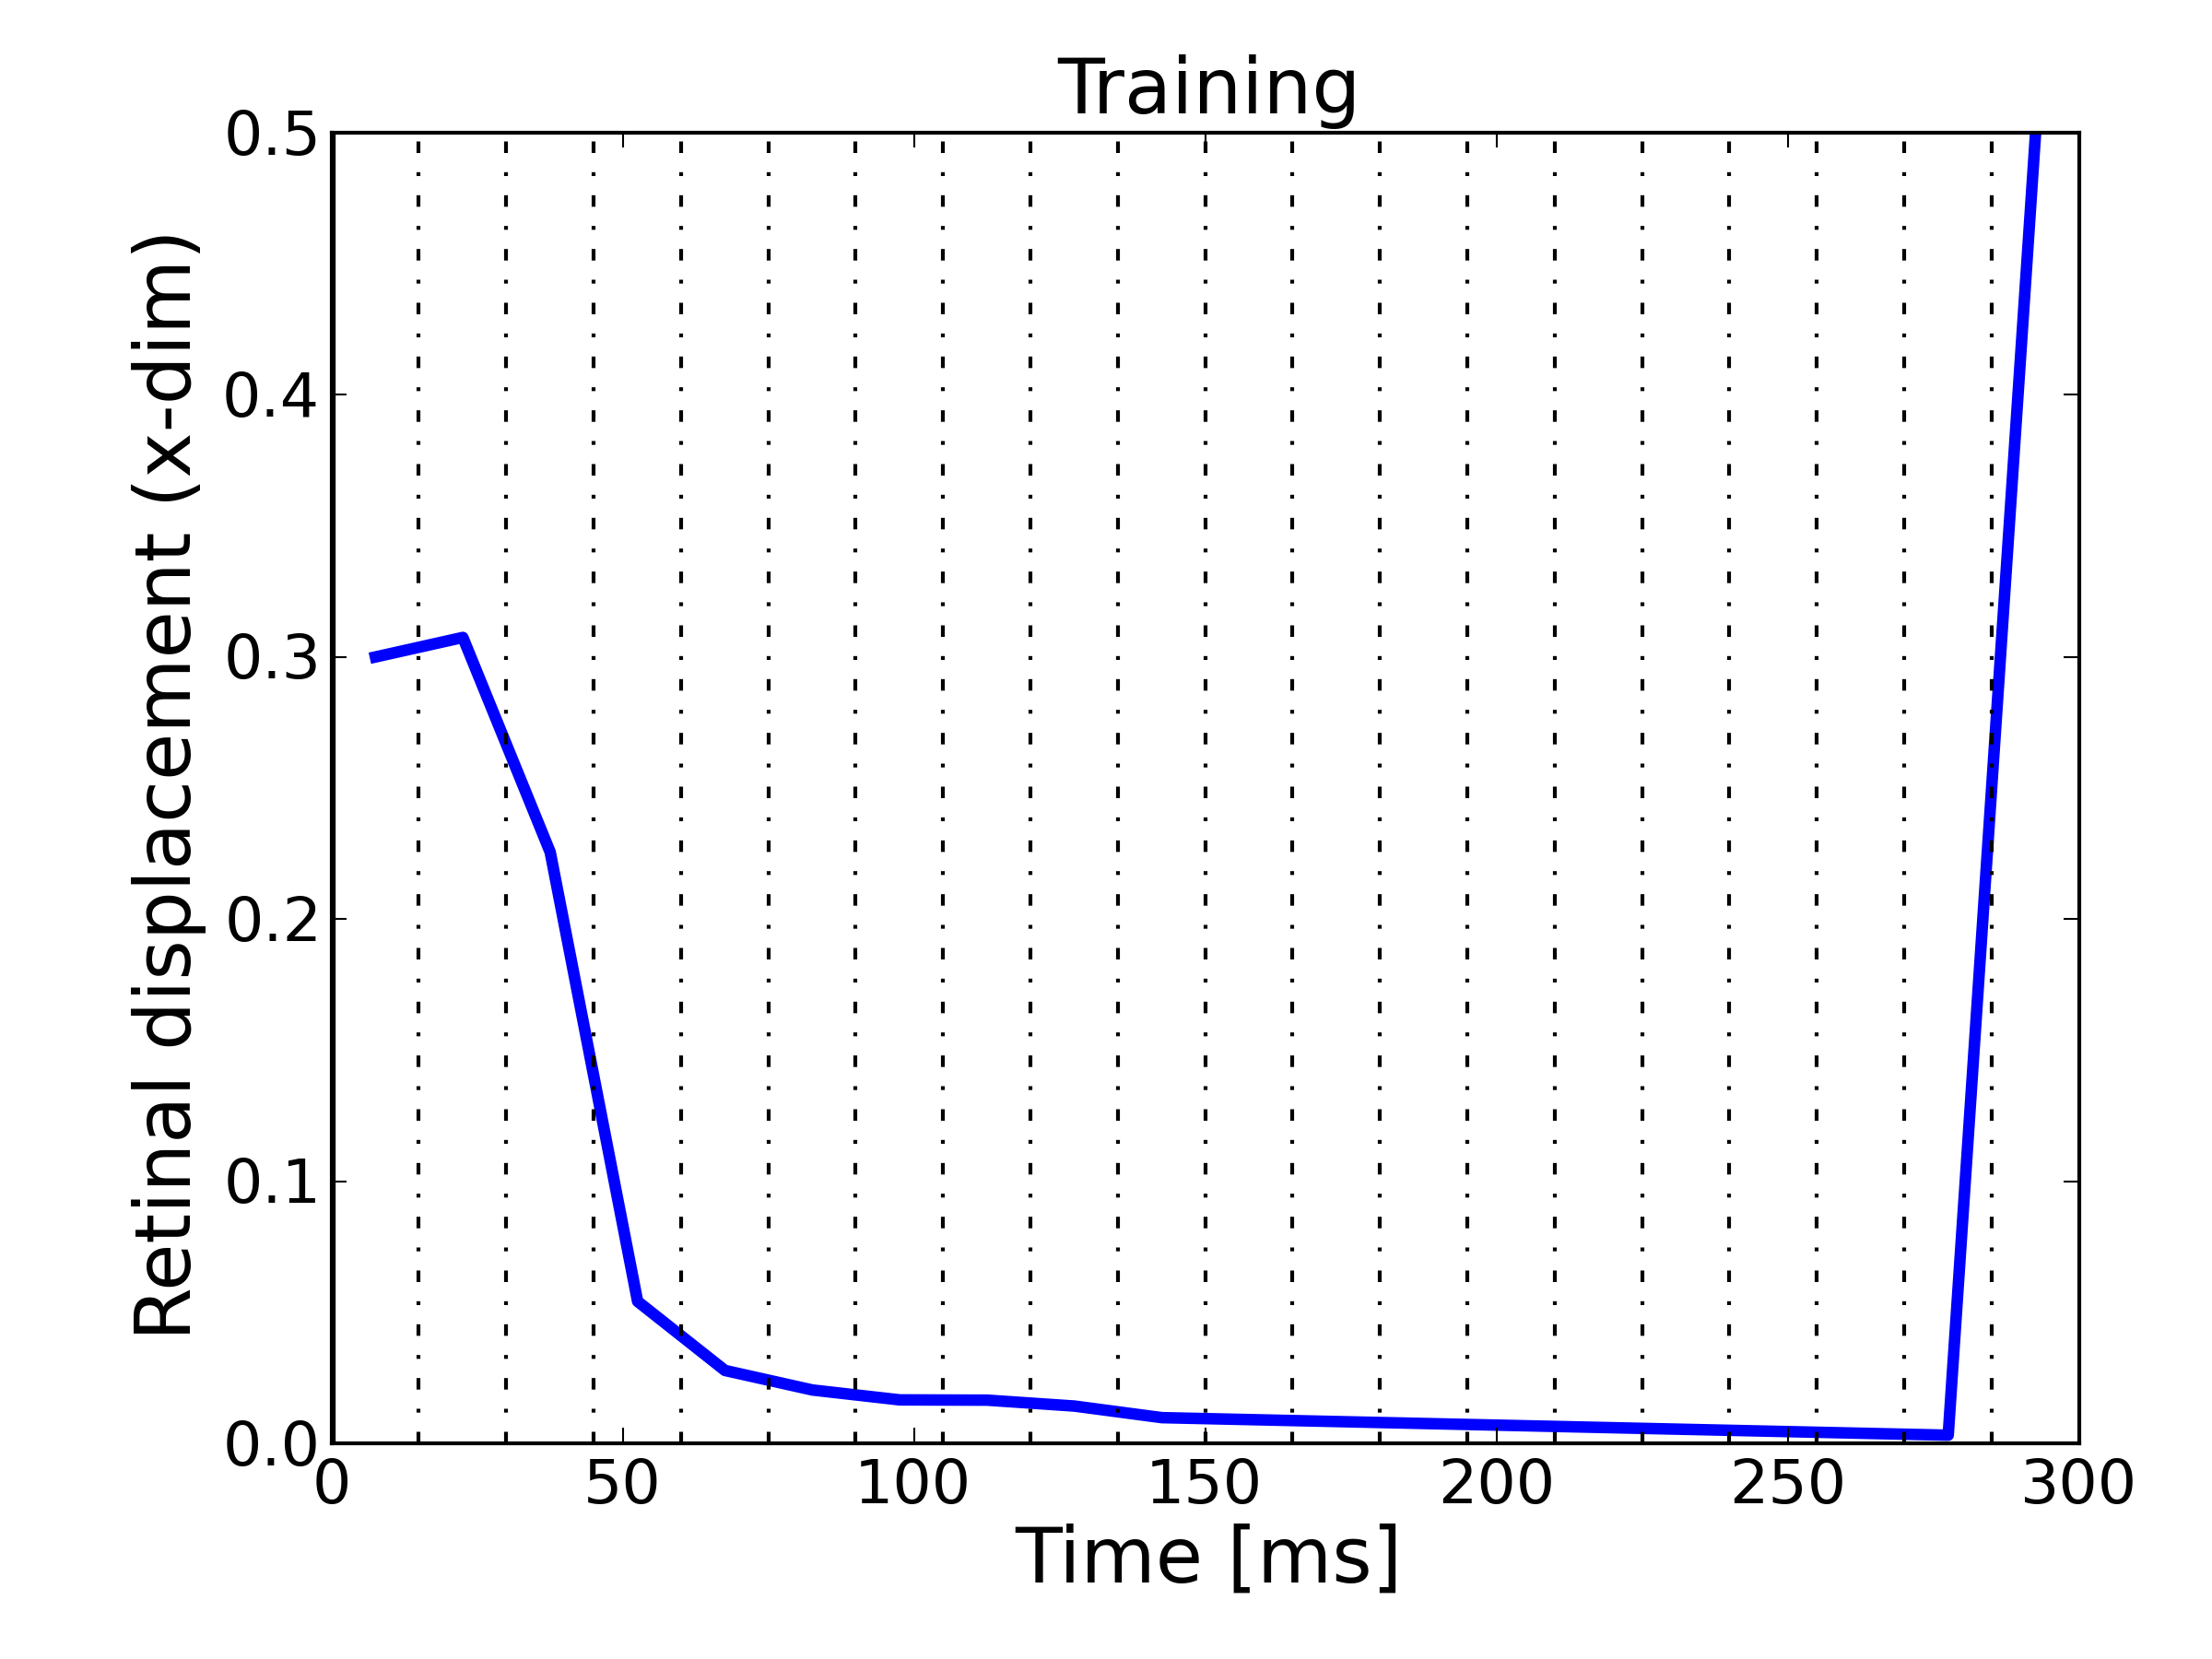
\includegraphics[width=0.4\textwidth]{\foldername/mpn_displacement} \end{figure}
%\end{tabular}


\begin{tabular}{cc}
	\includegraphics[width=0.4\textwidth]{\foldername/rasterplot_mpn_in_and_out_xpos}
	& 
	\includegraphics[width=0.4\textwidth]{\foldername/rasterplot_mpn_in_and_out_vx}
	\\
	\includegraphics[width=0.4\textwidth]{\foldername/training_sequence}
	&
	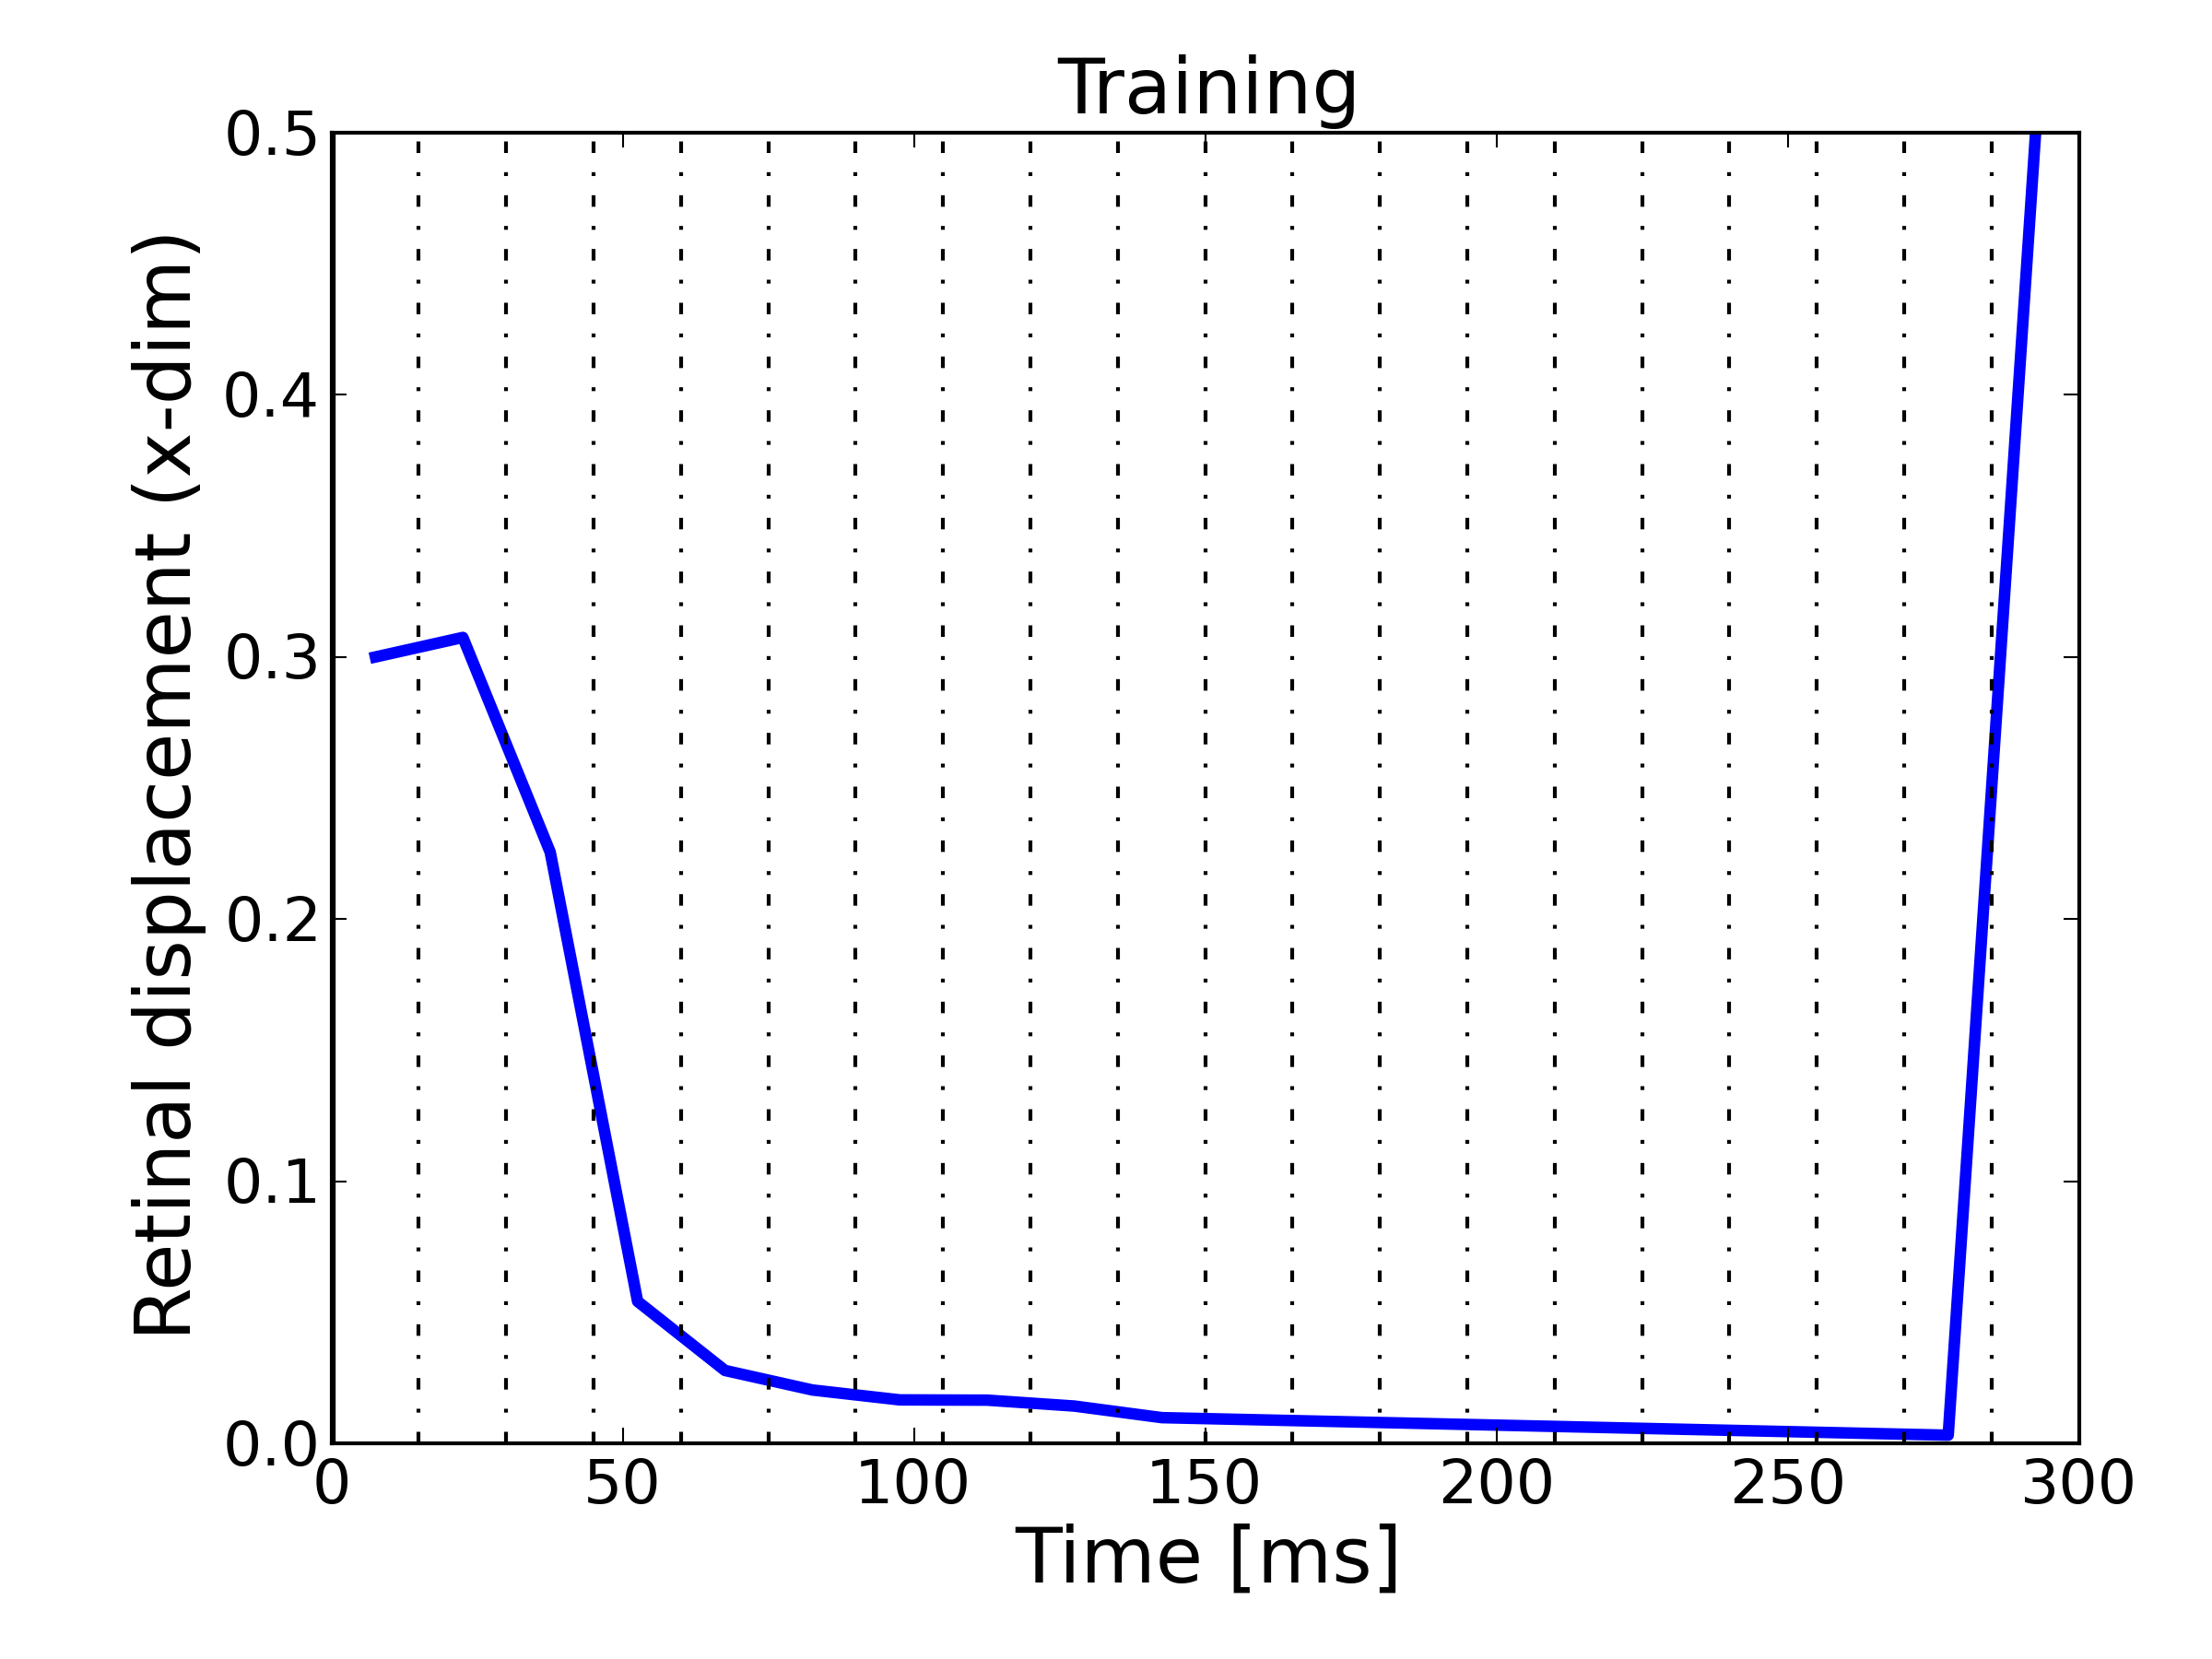
\includegraphics[width=0.4\textwidth]{\foldername/mpn_displacement}  
	\\
	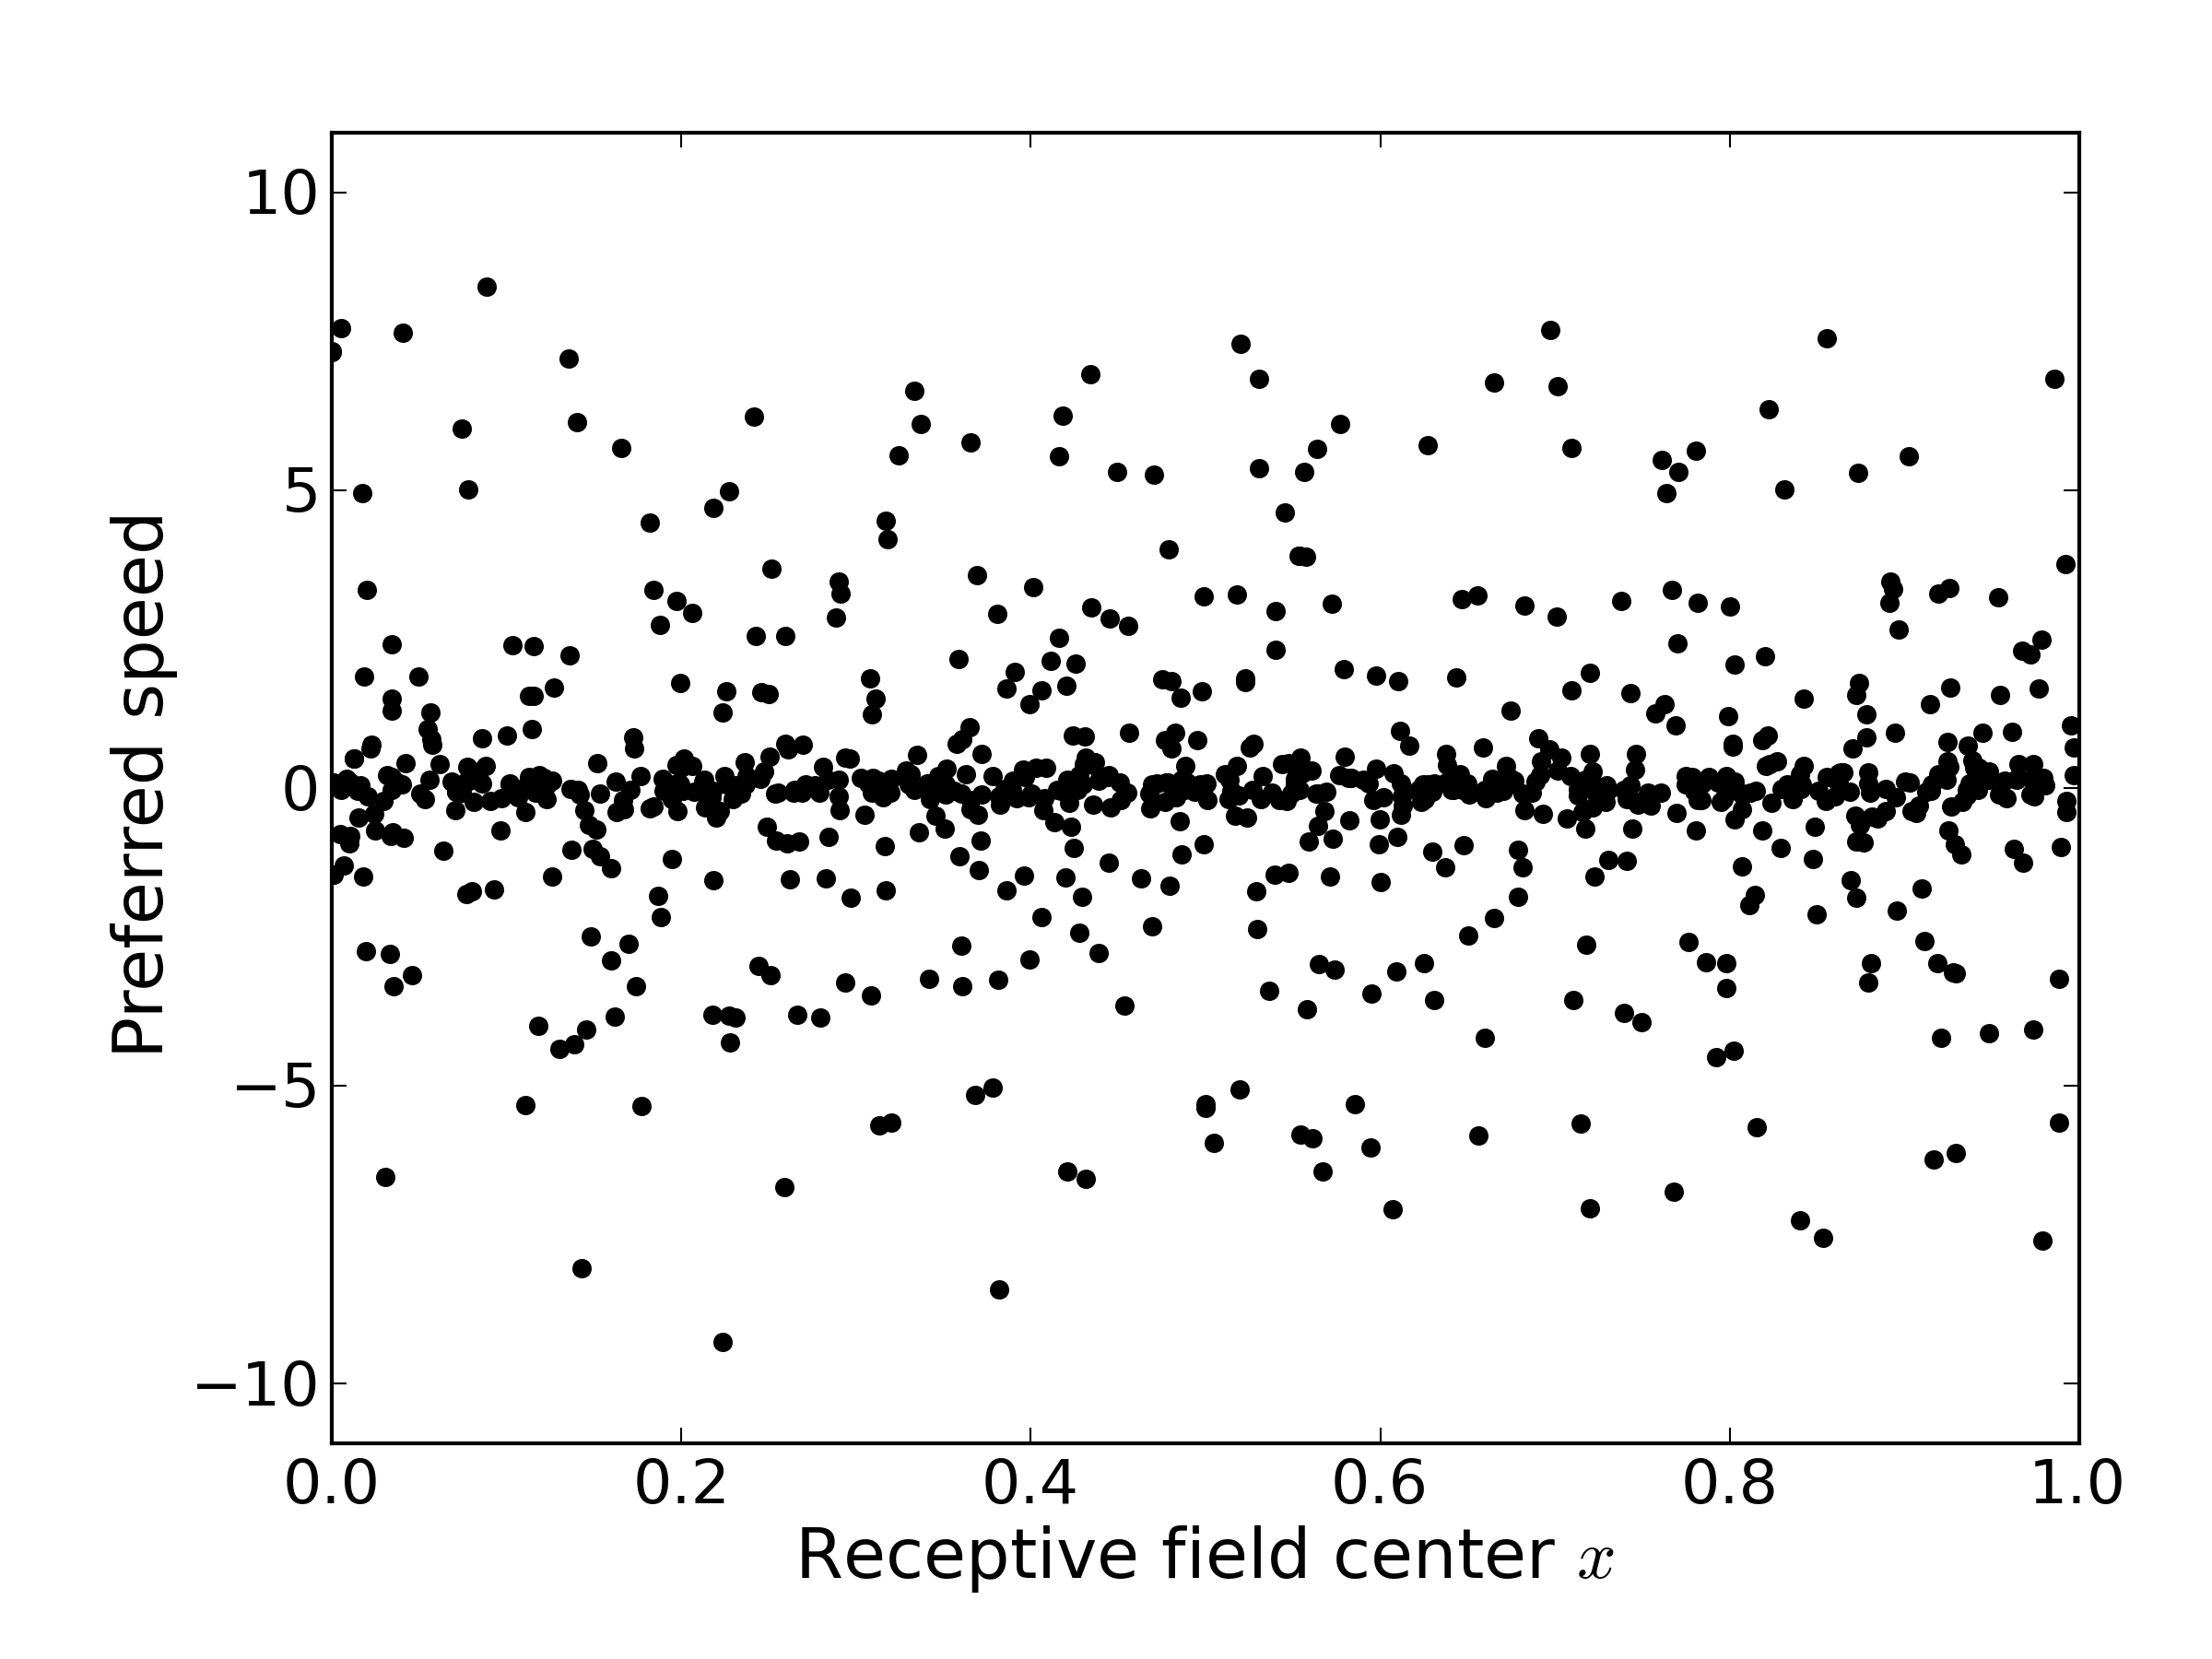
\includegraphics[width=0.4\textwidth]{\foldername/tuning_space} 
	&

\end{tabular}




\end{document}


